\begin{proof}
\begin{small}


Denote edge $e \in E$ by $e = (e_x , e_y )$.
Let $M'$ be any perfect matching in G (not necessarily in $E _\ell$ ).
Since every $v \in V$ is covered exactly once by M we
have $$w(M') = \sum _{e \in M'}w(e) \leq \sum _{e \in M'} (\ell(e_x ) + \ell(e_y )) = \sum _{v\in V} \ell(v)$$.
So $\underset{{v\in V}}{\ell(v)}$ is an \textbf{upper-bound} on the cost of any perfect matching.
Now let M be a perfect matching in $E_\ell$ . Then
$$w(M) = \underset{{e\in M}} w(e) = \underset{{v\in V}} \ell(v)$$
So $w(M')\leq w(M)$ and M is optimal.
\end{small}
\end{proof}

\begin{frame}{Improving Labellings}
Let $\ell$ be a feasible labeling.
We define neighbor of $u \in V$ and set $S \subseteq V$ to be
$$N_\ell (u) = {v\mbox{ } |\mbox{ } (u, v) \in E_\ell }$$
$$N_\ell (S) = \underset{u\in S}{\cup} N_\ell (u)$$
Let $S \subseteq X$ and $T = N_\ell (S) = Y$ . Set $$\alpha_\ell =\underset{x\in X,y \notin T}{ min} \{\ell(x) + \ell(y) - w(x, y)\}$$ and
\begin{equation*}
\ell'(v)=
\left\{ \begin{array}{ll}
\ell(v)-\alpha_\ell  \qquad \quad   & \mbox{ if } v\in s\\
\ell(v)+\alpha_\ell    &  \mbox{ if }v\in T\\
\ell(v)              &  \mbox{ otherwise }
\end{array}\right.
\end{equation*}
\end{frame}


\begin{frame}{Proof of Correctness}
\textbf{LEMMA 1}: If M is a matching and P is an augmenting path relative to M, then
$ M\oplus P$  is a matching, and $| M \oplus P | = | M | + 1 $. 
Fig. 1 denotes a graph G with a matching M and augmenting path P along with the matching $M \oplus P$.\\
\begin{figure}[h!]
\centering
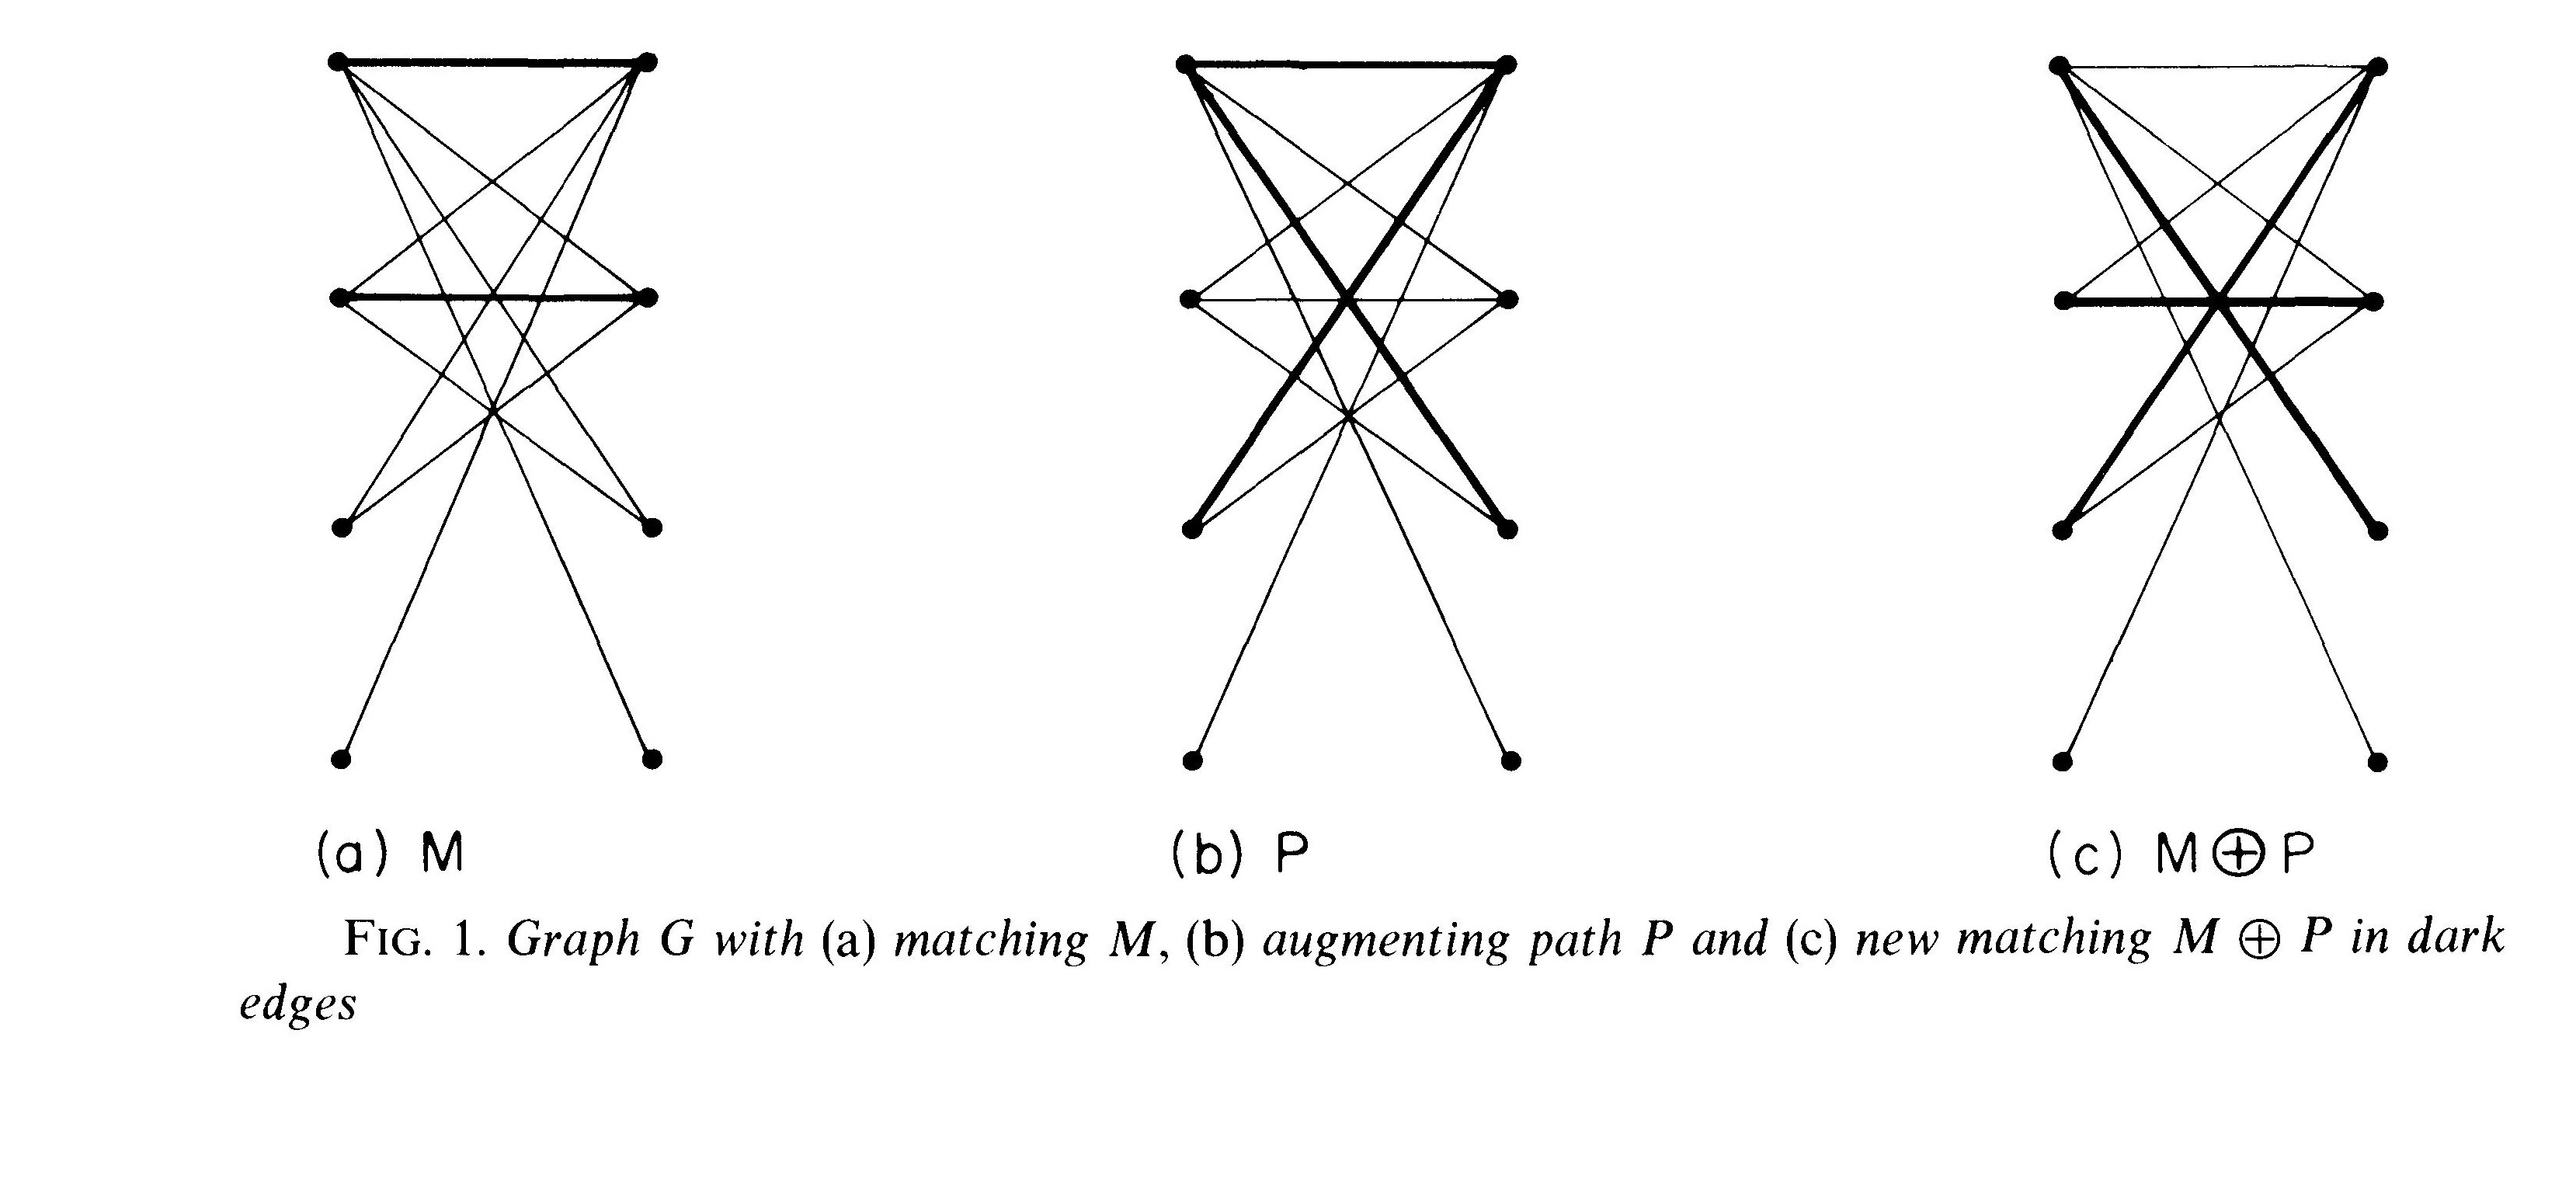
\includegraphics[width=1\textwidth]{graph}
\end{figure}
\end{frame}

\begin{proof} Let M be the maximum matching.On the contrary let us assume that there exists an augmenting path with respect to M. If we augment this path with M then we will get a matching of size one greater than size of M. So M cannot be the maximum matching.
\end{proof}

\begin{proof} Let $\ell$ be the length of shortest augmenting path.Let each path be of length $\ell$.The number of vertices covered by each path will be $\ell+1$.As the total number of vertices is bounded by n we have $$(s-r)(\ell +1) \leq n.$$
On simplification we get $$\ell \leq \frac{n}{s-r}-1$$
\end{proof}


\begin{proof}
 Let $N=(M \oplus P)\oplus P'$. Then $M \oplus N = P \oplus P'$. Now since $|N|=|M|+2$ there must exist two vertex disjoint augmenting paths with respect to M. Let $P1$ and $P2$ be the two augmenting paths. Since these are also vertex disjoint, $|P \oplus P'|$ will atleast be equal to $|P1|+|P2|$.
As P is the shortest augmenting path with respect to M, the following relation follows $$|M \oplus N|=|P\oplus P'|=|P|+|P'|-2|P \cap P'| \geq |P1|+|P2| \geq 2|P|$$. Simplifying we get $$ |P'| \geq |P|+2|P \cap P'|$$
\end{proof} 


\begin{proof}
\begin{itemize}

\item Suppose that in some phase we augmented the current matching by maximal set of vertex disjoint augmenting paths of length $k$. This yields a new matching $M'$.
\item Let P' be an augmenting path with respect to the new matching.If $P'$ is vertex disjoint from each path in the previous set of paths then it must have length strictly more than $k$ as it would contradict the statement that we had a maximal set of vertex disjoint paths of length $k$ in the previous iteration.
\end{itemize}
\end{proof}

\begin{frame}
\begin{proof}
\begin{itemize}

\item If it shares the vertex with some path in the previous chosen set of paths then it must have atleast one edge in common with $M'$ since every vertex in P is matched in $M'$.
\item Hence $P\cap P'$ is atleast one, so from above theorem $$|P'| \geq |P|+2|$$
\end{itemize}
\end{proof} 
\end{frame}

\begin{proof}
Let us assume that  $|P| = |Q|$ and P and Q are not node disjoint i.e $P\cup Q \neq \phi$.\\
From above \textbf{theorem} we have $P\cup Q = \phi$ as $|P| = |Q|$ i.e they are edge disjoint. Assume that P and Q share a common node v. Then they must share an edge between them contradicting $P \cap Q = \phi.$ Therefore, P and Q are also node-disjoint.
\end{proof} 

\begin{proof}
\begin{itemize}

\item Let A,B be two sets of a bipartite graphs.Denote by $A_0 , B_0$ the sets of M -unsaturated vertices in A, B respectively.Let $|V|=n$ and $|E|=m$.
\item Consider a new directed graph H on the vertex set $A \cup B$ and edge set E.
Edges which are in M are directed $A \rightarrow B$ and edges not in M are directed $B \rightarrow A$.
\item First we will use breadth-first-search BFS to find the length k of a shortest path from $B_0$ to $A_0$.Simultaneously, we produce the sequence of disjoint layers $B_0 = L_0 , L_1 , L_2 , ..., L_k \subseteq A_0$ where
\begin{enumerate}
\item for all $0 \leq i < k, L_i$ is the set of vertices at distance i from $B_0$.
\item $L_k$ is the subset of $A_0$ which is at distance k from $B_0$ .
\end{enumerate}
\end{itemize}
\end{proof}

\begin{proof}
\begin{itemize}
\begin{small}


\item To avoid multiple BFS's from each vertex in $B_0$ , we add a super-vertex $\beta$ and draw edges from it to all vertices of $B_0$ .
\item Start a BFS from $\beta$ to get distance of $\beta$ from $A_0$ . Subtract one to get length of shortest path from $B_0$ to $A_0$ . This takes $\mathcal{O}$(m) time.
\item Now consider a modified DFS which starts at a vertex $v \in B_0$ and stops as soon as it reaches a vertex say w in $L_k$ and outputs this $v \rightarrow w $path.
\item Add this M -augmenting path to a set say $\mathcal{F}$ and delete all vertices visited in the modified DFS. Redo the whole procedure now starting at another vertex in $B_0$ .
\item Continue until all vertices of $B_0$ are explored. This clearly gives us a maximal family of vertex-disjoint shortest-length augmenting paths.
\item Since we do not go to a depth of more than 'k' in DFS all the edges in graph are not traversed.
\item Let $m_i$ be the number of edges visited in the $i^{th}$ DFS which takes $\mathcal{O}(m_i)$ time. Noting that $m \geq \sum m_i$ , the time taken is $\mathcal{O}(m)$.
\end{small}
\end{itemize}
\end{proof}

The optimality of solution depends on who proposes in the algorithm. If men propose to women then the solution is man optimal i.e men get the best possible female partners it can have in any stable matching. It also means that women get the worst partner she can have in any stable matching. The solution does not depend upon which man proposes first. It will always give the same man optimal matching.


\begin{frame}{GS Lists}
\begin{enumerate}

\item Above mentioned algorithm gives only one of the many possible stable matchings. 
\item In order to get all possible matchings,we need to construct the GS list.GS lists are computed using the modified version of this algorithm.
\item In the above algorithm after the first iteration we get a tentative matching.
\item In the subsequent iterations the matching with respect to men can only improve.
\end{enumerate}
\end{frame}

\begin{frame}{GS Lists}
\begin{enumerate}

\item So in the preference list of men for women we may as well delete the entries which are after the women to which a man is currently matched.
\item In particular the extended version reduces the preference list by eliminating certain pairs that can be readily identified as not belonging to any stable matching.
\item In the extended algorithm when a man `m' proposes to a women `w', the proposes is always accepted.
\item For if `w' already held a proposal from someone she prefers to `m' then the pair (m,w) would already have been deleted.
\item This algorithm can be used in cases when number of men and women are not equal and also when some men give incomplete preferences of women or vice-versa.

\end{enumerate}
\end{frame}


\begin{algorithm}[H]



\caption{Modified algorithm}
Assign each person to be free\\
\While {some man m is free}{
	$ w :=$ first women on m's list
	if{ some man p is engaged to w}{
		assign p to be free\\
		assign m and w to be engaged to each other\\
		\For {each successor m' of m on w's list}			{
 			delete pair (m',w)
		}
	}
}

\end{algorithm}


\begin{algorithm}[H]%{Pseudo Code}
\begin{scriptsize}
Start with any feasible labeling $\ell$ and some matching M in $E_\ell$.\\
\While{M is not perfect}{

 Find an augmenting path for M in $E_\ell$ ;
(this increases size of M)\\
 \If {no augmenting path exists}{
 Improve $\ell$ to $\ell'$ such that $E_\ell \subset E_\ell'$.\newline
 Go to 1.}
 }
\begin{itemize}
\item In each step of the loop we will either be increasing the size of M or $E_\ell$ so this process must terminate. 
\item When the process terminates, M will be a perfect matching in $E_\ell$ for some feasible labeling $\ell$.So, by the Kuhn-Munkres theorem, M will be a max-weight matching.
\end{itemize}
To find an initial feasible labeling we use:
$$ \forall y \in Y, \ell(y) = 0,\forall x \in X, \ell(x) = \underset{y \in Y}{max} \{w(x, y)\}$$
With this labeling it is obvious that
$$ \forall x \in X, y \in Y, w(x) \leq \{\ell(x) + \ell(y)\}$$
\end{scriptsize}
\end{algorithm}


\begin{frame}{Labellings \& Equality Graphs}
\begin{itemize}


\item A vertex labeling is a function $\ell$ : V $\rightarrow$ R. \newline
A feasible labeling is one such that $$\ell(x) + \ell(y) \geq w(x, y),\forall x \in X, y \in Y$$.
\item The Equality Graph with respect to $\ell$ is G = (V, E$_l$ ) where
$$E_\ell = \{(x, y) : \ell(x) + \ell(y) = w(x, y ) \}$$
\end{itemize}
\end{frame}


\begin{frame}

\begin{theorem}\label{my theorem}
If $\ell$ is feasible and M is a Perfect matching
in E$_\ell$ then M is a max-weight matching.%\\ \newline
\end{theorem}


\begin{theorem}{Kuhn-Munkres Theorem} : If $\ell$ is feasible and M is a
perfect matching in $E_\ell$ then M is a max-weight matching.
\end{theorem}
\begin{itemize}
\item The KM theorem transforms the problem from an optimization problem of finding a max-weight matching into a combinatorial one of finding a perfect matching.
\item  It combinatorializes the weights.
\end{itemize}
\end{frame}
